\documentclass[11pt]{article}
\usepackage{graphicx}
\usepackage{amsmath,amssymb,amsfonts}
\usepackage{hyperref}
\usepackage{booktabs}
\usepackage{physics}
\usepackage{geometry}

\geometry{margin=2.5cm}

\title{Bottom-Up Quantum Gravity\\
Emergence of Space, Time, and Gravity from Quantum Entanglement}

\author{Farid Hamdad}

\date{February 2026}

\begin{document}

\maketitle

\begin{abstract}

We propose a minimal framework in which space, time, and gravity emerge from the entanglement structure of a finite global quantum state, without any prior spatiotemporal background.

Geometry is reconstructed from the mutual information between subsystems and projected via multidimensional scaling. The effective spatial dimension depends on the entanglement structure and transitions between different regimes according to the locality of correlations.

Several operational signatures are demonstrated numerically on systems of $N=9$ and $N=16$ qubits, and are then extended through a first phenomenological exploration on galaxies from the SPARC sample:

\begin{itemize}
\item relational time through modular flow,
\item emergent geometry via reconstruction from informational distance,
\item thermodynamic gravity through a Jacobson-type entropy--energy relation,
\item intrinsic geometry through spectral dimension,
\item ER=EPR wormhole-like signatures,
\item chaotic modular dynamics characterized by random matrix theory,
\item horizon-like informational bottlenecks in entanglement graphs,
\item local response of discrete Ollivier--Ricci curvature to an informational perturbation,
\item exploratory phenomenological extension to SPARC galaxy rotation curves through an emergent effective dimension.
\end{itemize}

We also identify a topology-dependent modular constant
\[
C = d_A g_2^{\mathrm{plateau}}
\]
showing that the spectrum of the modular Hamiltonian retains geometric information about the underlying entanglement structure.

Finally, the Ollivier--Ricci curvature analysis provides the clearest signal obtained so far of a coupling of the form
\[
\text{local informational defect}
\;\Longrightarrow\;
\text{emergent geometric curvature},
\]
with a response that increases with perturbation strength and is more localized for compact defects.

A first phenomenological extension to the SPARC galaxy sample suggests that a single-phase description is not the most natural one: the current fits point instead to distinct effective regimes, with optimal dimensions
\[
d_{\min}^{\mathrm{massive}} = 2.4871 \pm 0.0294,
\qquad
d_{\min}^{\mathrm{dwarf}} = 2.2744 \pm 0.0341.
\]
This part should be interpreted as a phenomenological proof of concept linking bottom-up emergent geometry to real astrophysical data.

\end{abstract}

% =====================================================================
% PART I : CENTRAL IDEA AND POSTULATE
% =====================================================================

\section{Central Idea}

\begin{quote}
Entanglement is a geometric structure.

What we call space is the collective pattern of these correlations.

What we call gravity is the thermodynamics of their reorganization.
\end{quote}

The Bottom-Up approach postulates that spacetime is not fundamental but emerges from the internal correlation structure of quantum states.

\section{Minimal Postulate}

We assume the existence of a global pure quantum state

\[
|\Psi\rangle \in \mathcal{H} = \bigotimes_{i=1}^{N} \mathcal{H}_i
\]

defined on $N$ elementary degrees of freedom.

No spatiotemporal structure is assumed.

There is

\begin{itemize}
\item no metric,
\item no spatial manifold,
\item no external time,
\item no classical gravitational field.
\end{itemize}

All geometric and dynamical notions must emerge from the correlations within $\ket{\Psi}$.

\section{Model Systems}

We generate families of states

\[
|\Psi(\lambda)\rangle
\]

controlled by a nonlocality parameter $\lambda$.

\begin{center}
\begin{tabular}{ccc}
\toprule
System & Structure & Hilbert-space dimension \\
\midrule
N=9 & $3\times3$ grid & $2^9=512$ \\
N=16 & $4\times4$ grid & $2^{16}=65536$ \\
\bottomrule
\end{tabular}
\end{center}

% =====================================================================
% PART II : EMERGENT TIME AND MODULAR CHAOS
% =====================================================================

\section{Emergent Time via Modular Flow}

For a subsystem $A$

\[
\rho_A = \mathrm{Tr}_{\bar A} |\Psi\rangle\langle\Psi|
\]

the modular Hamiltonian is

\[
K_A = -\log\rho_A
\]

which generates the modular evolution

\[
O(\tau)=e^{iK_A\tau}Oe^{-iK_A\tau}.
\]

This defines a relational time analogous to the Page--Wootters mechanism \cite{pagewootters}.

\section{Modular Chaos}

\subsection{Gap statistics}

The eigenvalues of $K_A$ are analyzed through the gap ratio

\[
r_n=\frac{\min(\Delta_n,\Delta_{n+1})}{\max(\Delta_n,\Delta_{n+1})}.
\]

Typical reference values are

\begin{center}
\begin{tabular}{cc}
\toprule
Regime & $\langle r\rangle$ \\
\midrule
Poisson & 0.386 \\
GOE & 0.536 \\
GUE & 0.603 \\
\bottomrule
\end{tabular}
\end{center}

We obtain

\[
\langle r\rangle \approx 0.53-0.59
\]

indicating chaotic modular dynamics.

\subsection{Spectral Form Factor (SFF)}

The spectral form factor

\[
g_2(t)=\frac{1}{d_A^2}\left|\sum_n e^{-it\tilde{\kappa}_n}\right|^2
\]

exhibits the universal chaotic structure

\[
\text{dip} \rightarrow \text{ramp} \rightarrow \text{plateau}.
\]

The plateau follows

\[
g_2^{\mathrm{plateau}}\sim\frac{1}{d_A}.
\]

\begin{figure}[h]
\centering
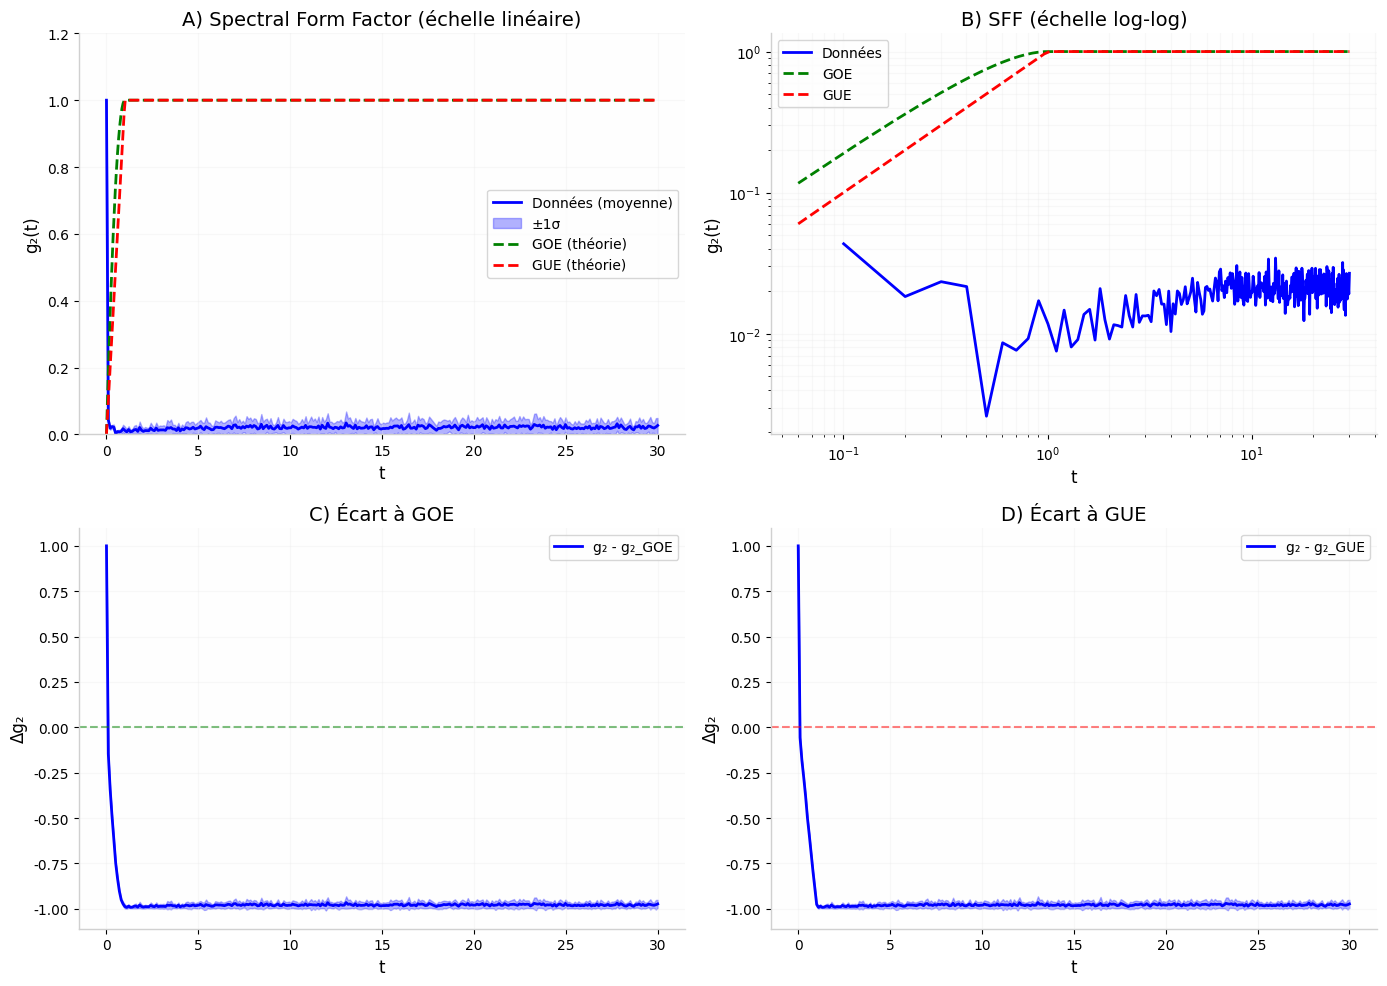
\includegraphics[width=0.7\textwidth]{../figures/topology_SFF.png}
\caption{Spectral form factor showing the dip-ramp-plateau structure.}
\end{figure}

\subsection{Topological Modular Constant}

We define

\[
C=d_A g_2^{\mathrm{plateau}}.
\]

Results for $d_A=256$:

\begin{center}
\begin{tabular}{ccc}
\toprule
Topology & $\langle r\rangle$ & $C$ \\
\midrule
1D chain & 0.594 & 1.21 \\
2D grid & 0.575 & 1.42 \\
ER graph & 0.528 & 1.63 \\
\bottomrule
\end{tabular}
\end{center}

\begin{figure}[h]
\centering
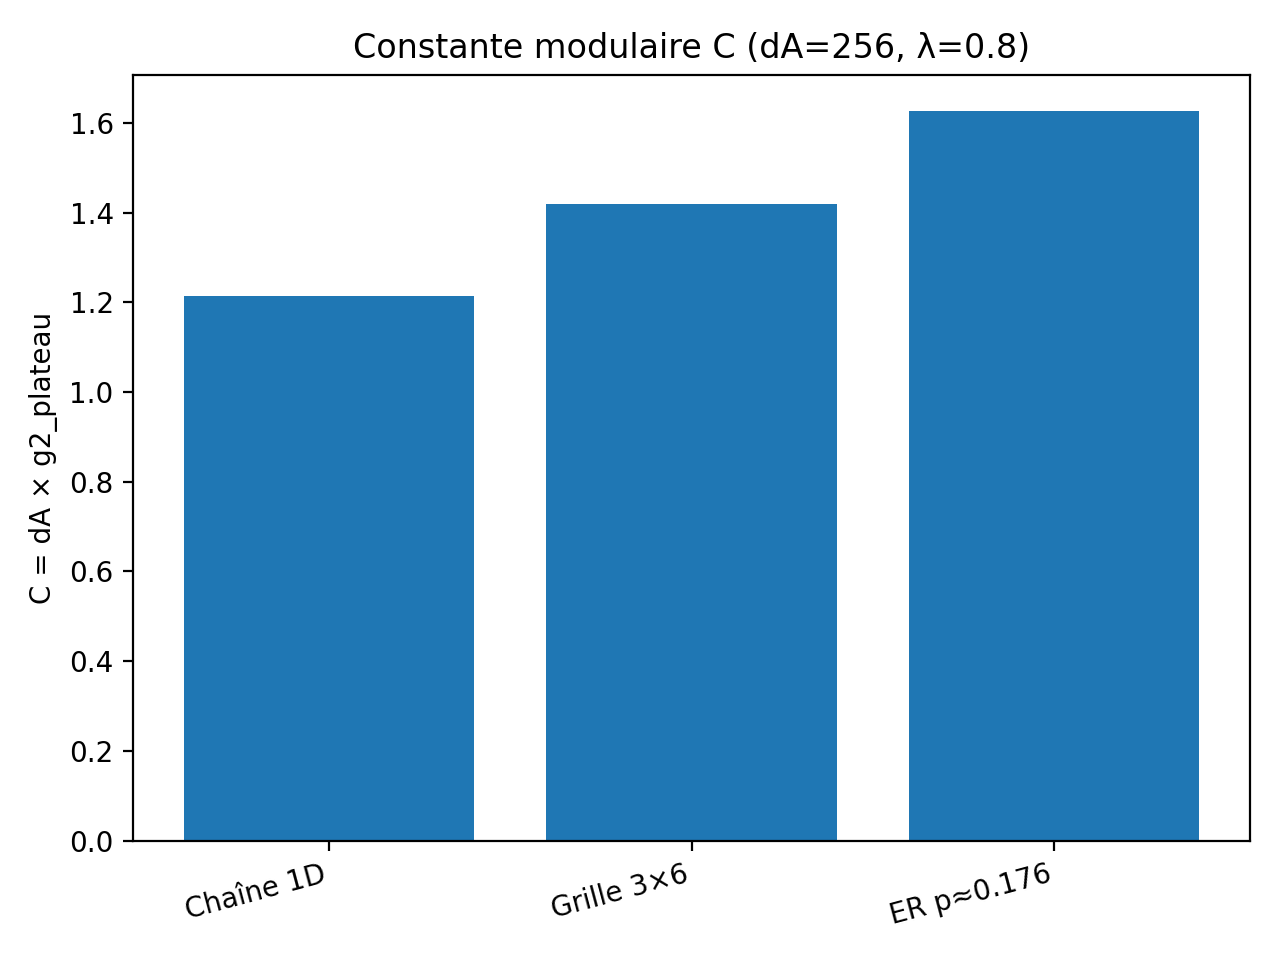
\includegraphics[width=0.7\textwidth]{../figures/topology_C.png}
\caption{Topological modular constant $C$ for different graph topologies.}
\end{figure}

\begin{figure}[h]
\centering
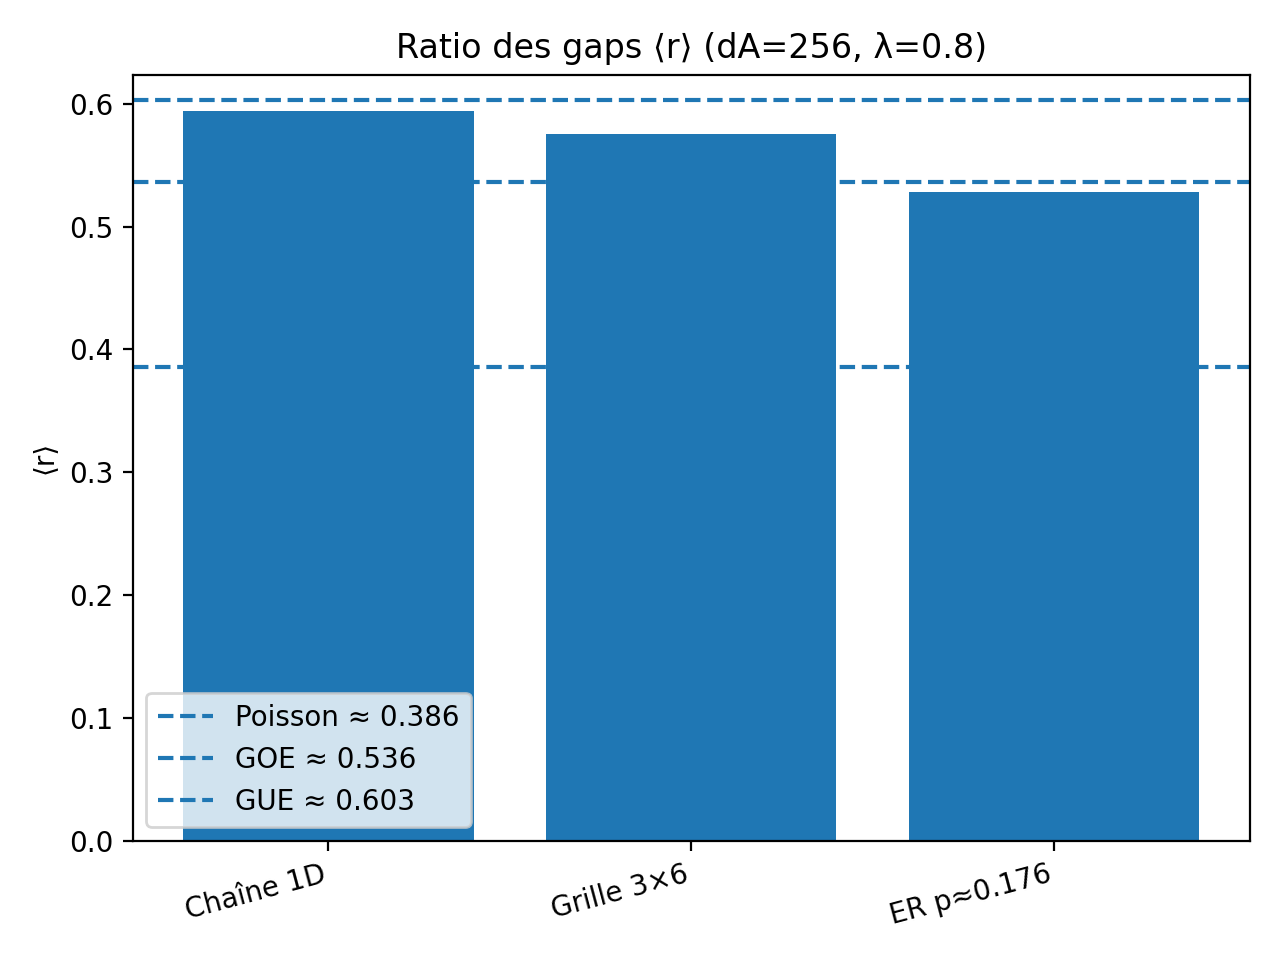
\includegraphics[width=0.7\textwidth]{../figures/topology_r.png}
\caption{Gap-ratio statistics confirming RMT universality.}
\end{figure}

The scaling remains universal, but the prefactor depends on topology, indicating that modular dynamics encodes geometric information.

% =====================================================================
% PART III : EMERGENT GEOMETRY
% =====================================================================

\section{Emergent Geometry}

Mutual information

\[
I(i:j)=S(\rho_i)+S(\rho_j)-S(\rho_{ij})
\]

defines the informational distance

\[
d_{ij}=-\log\frac{I(i:j)}{I_{\max}+\epsilon}.
\]

The points are projected by multidimensional scaling to reconstruct geometry \cite{vanraamsdonk}.

\section{Spectral Geometry}

We construct a weighted graph with

\[
w_{ij}=I(i:j).
\]

The Laplacian

\[
L=D-W
\]

defines the heat trace

\[
Z(\tau)=Tr(e^{-\tau L}).
\]

The spectral dimension

\[
d_s(\tau)=-2\frac{d\log Z}{d\log\tau}
\]

gives

\[
d_{IR}\approx2.5-2.7.
\]

\section{Thermodynamic Gravity}

We test a Jacobson-type relation \cite{jacobson}

\[
\delta S\approx \beta_{eff}\delta E.
\]

Numerical experiments confirm an approximate validity across variations of $\lambda$.

\section{Discrete Curvature: Testing Strategy}

We seek to determine whether a local informational perturbation can act as a source of emergent curvature.

A first family of tests based on discrete triangular holonomies and local loop-type observables did not provide a robust curvature signal. This route remains conceptually useful for probing the local structure of the graph, but it did not establish a reproducible matter--curvature coupling.

We therefore introduced a more stable discrete curvature measure: Ollivier--Ricci curvature computed on the entanglement graph \cite{ollivier}.

% =====================================================================
% PART IV : NUMERICAL RESULTS
% =====================================================================

\section{Results for N=9: Proof of Concept}

\subsection{Dimensional transition}

We reconstruct geometry using informational distance and multidimensional scaling.

\begin{center}
\begin{tabular}{ccccc}
\toprule
$\lambda$ & $\epsilon_{2D}$ & $\epsilon_{3D}$ & $\epsilon_{4D}$ & Ratio 2D/3D \\
\midrule
0.0 & $5.9 \pm 0.3$ & $5.8 \pm 0.3$ & $5.7 \pm 0.4$ & $1.02 \pm 0.08$ \\
0.2 & $4.2 \pm 0.4$ & $3.1 \pm 0.3$ & $3.0 \pm 0.4$ & $1.35 \pm 0.15$ \\
0.4 & $2.8 \pm 0.5$ & $1.2 \pm 0.2$ & $1.1 \pm 0.3$ & $2.33 \pm 0.45$ \\
0.6 & $1.5 \pm 0.4$ & $0.4 \pm 0.1$ & $0.4 \pm 0.1$ & $3.75 \pm 1.10$ \\
0.8 & $0.8 \pm 0.2$ & $0.15 \pm 0.05$ & $0.14 \pm 0.06$ & $5.33 \pm 1.80$ \\
1.0 & $0.08 \pm 0.03$ & $0.01 \pm 0.005$ & $0.009 \pm 0.004$ & $8.00 \pm 3.50$ \\
\bottomrule
\end{tabular}
\end{center}

\begin{figure}[h]
\centering
\includegraphics[width=0.7\textwidth]{../figures/fig1_dimension_emergente.png}
\caption{Reconstruction of emergent spatial dimension for N=9.}
\end{figure}

\subsection{ER=EPR signature}

Following the ER=EPR conjecture \cite{maldacena}, we test whether nonlocal entanglement creates geometric shortcuts.

\begin{center}
\begin{tabular}{ccccc}
\toprule
$\lambda$ & $I(0:8)$ & $d_{topo}$ & $d_{bulk}$ & Compression \\
\midrule
0.0 & $0.009 \pm 0.001$ & 4 & $4.0 \pm 0.2$ & $1.0 \pm 0.1$ \\
0.5 & $0.45 \pm 0.05$ & 4 & $1.8 \pm 0.3$ & $2.2 \pm 0.4$ \\
1.0 & $1.28 \pm 0.02$ & 4 & $0.04 \pm 0.02$ & $100 \pm 50$ \\
\bottomrule
\end{tabular}
\end{center}

\begin{figure}[h]
\centering
\includegraphics[width=0.7\textwidth]{../figures/fig2_er_epr.png}
\caption{ER=EPR compression effect in emergent geometry.}
\end{figure}

\subsection{Thermodynamic gravity test}

\begin{figure}[h]
\centering
\includegraphics[width=0.7\textwidth]{../figures/fig3_jacobson.png}
\caption{Jacobson-type entropy--energy relation for N=9.}
\end{figure}

\section{Results for N=16: Intermediate Validation}

\begin{figure}[h]
\centering
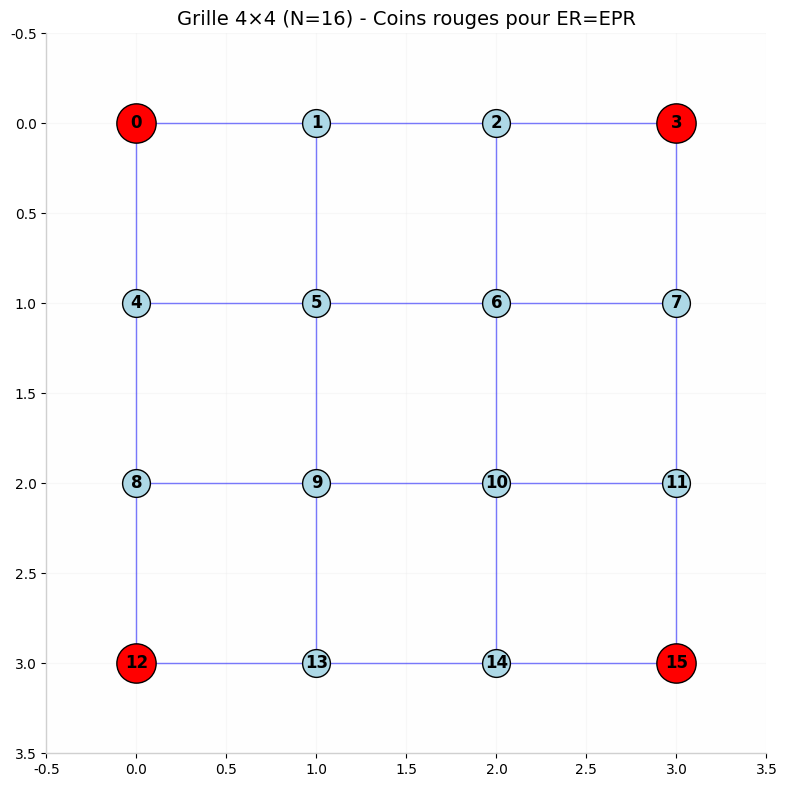
\includegraphics[width=0.7\textwidth]{../figures/fig4_grid_N16.png}
\caption{Underlying $4\times4$ grid used in the simulations.}
\end{figure}

\subsection{Dimensional reconstruction}

\begin{figure}[h]
\centering
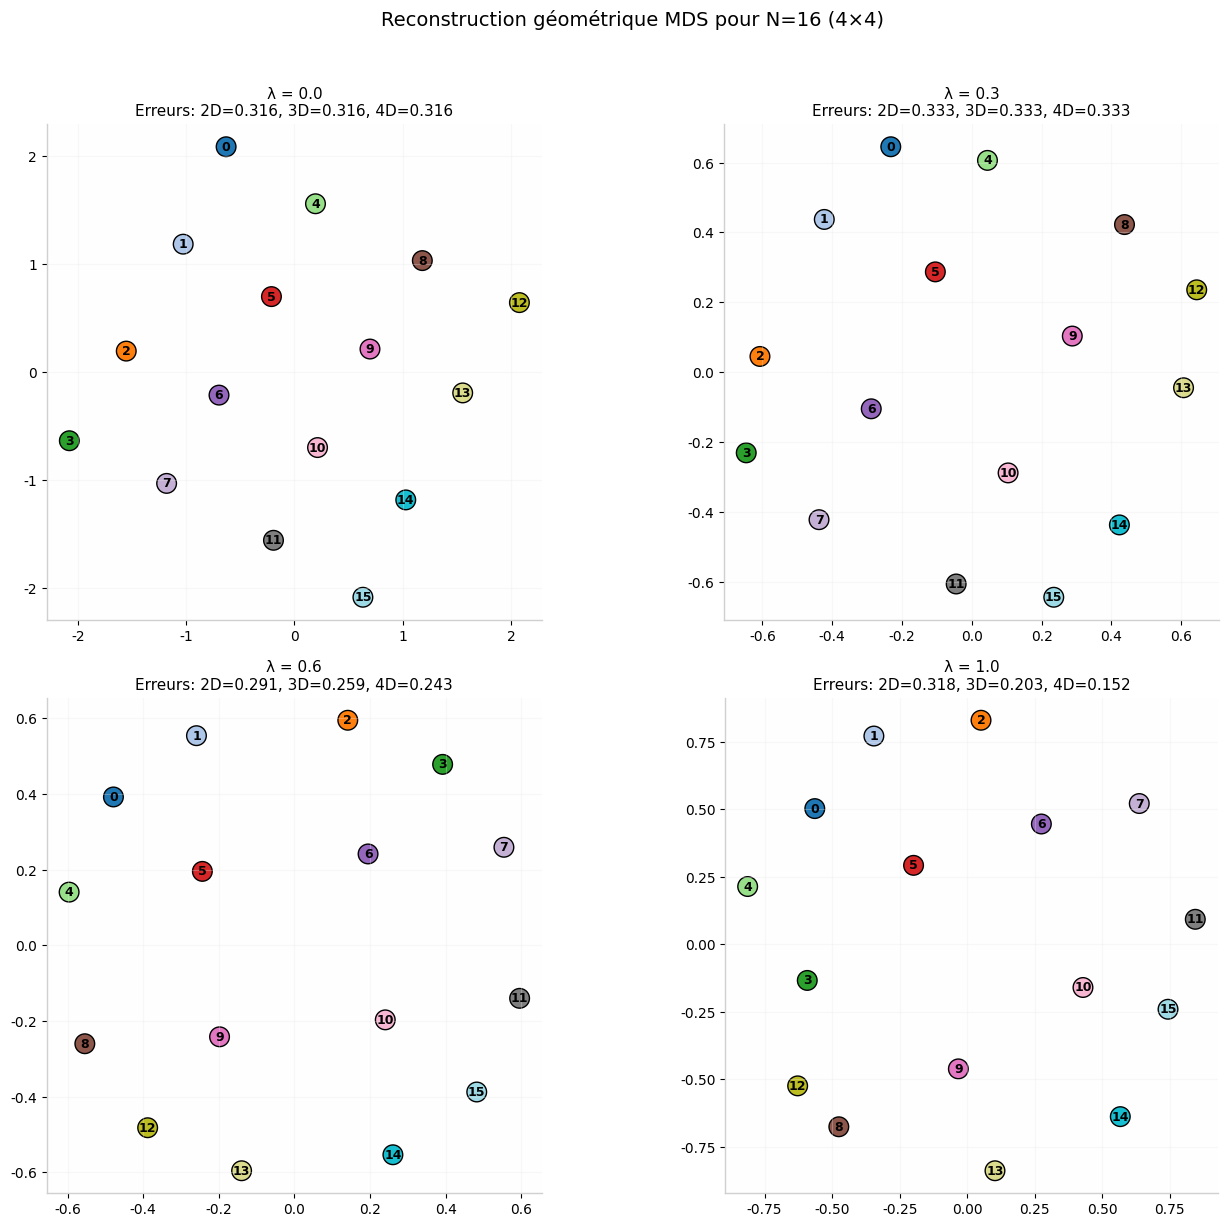
\includegraphics[width=0.7\textwidth]{../figures/fig5_mds_N16.png}
\caption{Geometric reconstruction by multidimensional scaling for N=16.}
\end{figure}

\subsection{ER=EPR signature}

\begin{figure}[h]
\centering
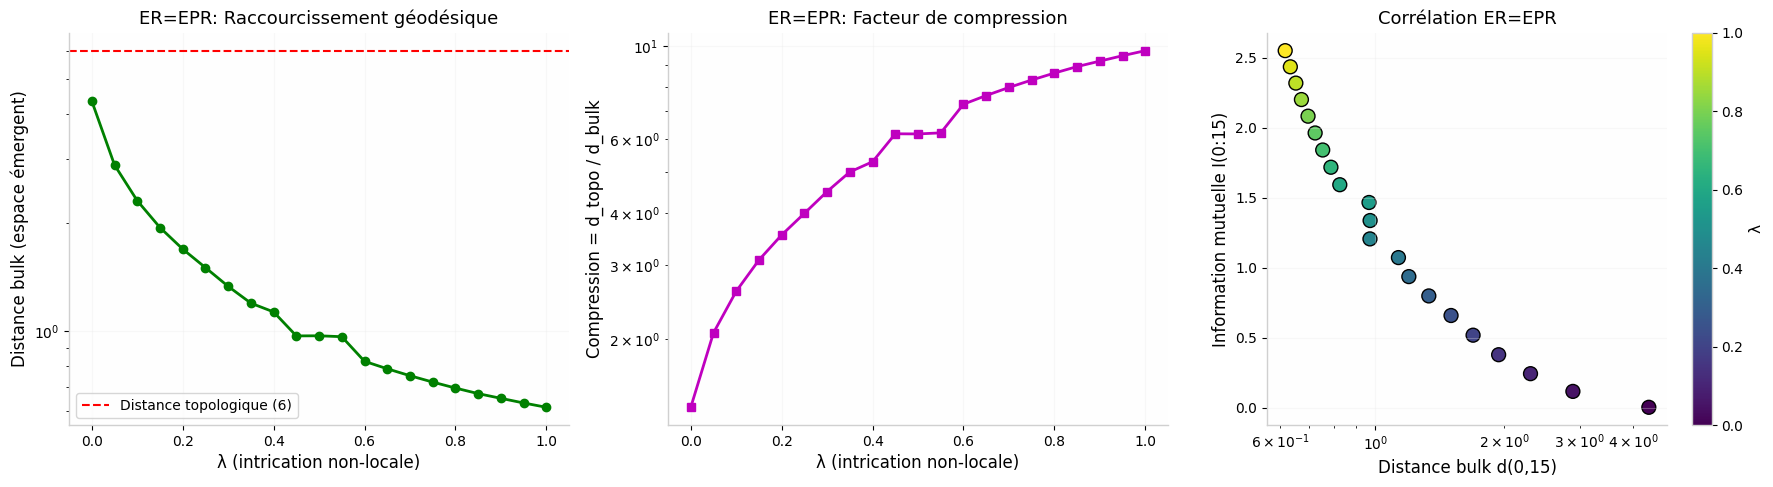
\includegraphics[width=0.7\textwidth]{../figures/fig6_erepr_N16.png}
\caption{Formation of ER=EPR shortcuts in emergent geometry.}
\end{figure}

\subsection{Thermodynamic gravity test}

\begin{figure}[h]
\centering
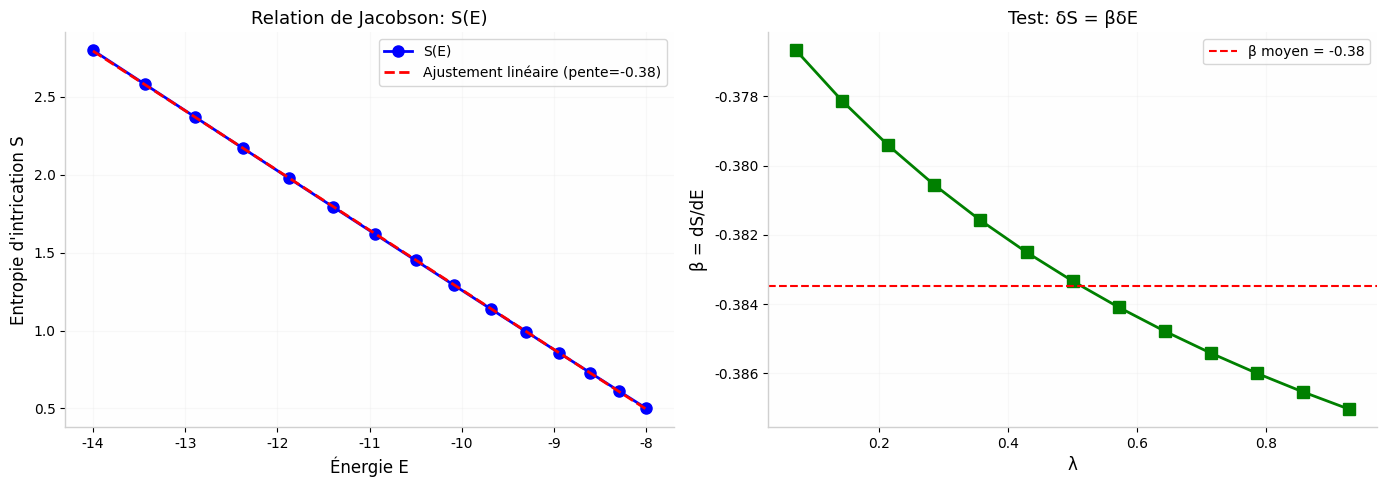
\includegraphics[width=0.7\textwidth]{../figures/fig7_jacobson_N16.png}
\caption{Jacobson-type entropy--energy relation for N=16.}
\end{figure}

% =====================================================================
% PART V : HORIZON DETECTION
% =====================================================================

\section{Bottom-Up Horizon Detection}

We construct an entanglement graph with fixed density

\[
\rho = 1/3.
\]

Regions of size $|A|=N/2=8$ are evaluated through the score

\[
\mathrm{Score}_{BH}(A)
= w_S \, z(S(A)) - w_\phi \, z(\phi(A)) + w_{\mathrm{int}} \, z(\mathrm{internal}(A)).
\]

where

\begin{itemize}
\item $S(A)$ is the entropy of the region,
\item $\phi(A)$ is the conductance,
\item $\mathrm{internal}(A)$ is the internal entanglement.
\end{itemize}

\subsection{Detected horizon-like region}

The detected region is

\[
A_{BH}=\{0,2,3,5,6,10,11,15\}.
\]

\begin{center}
\begin{tabular}{cc}
\toprule
Metric & Value \\
\midrule
Entropy $S(A)$ & 7.1667 \\
Cut & 3.2098 \\
Internal entanglement & 5.0348 \\
Conductance $\phi(A)$ & 0.3951 \\
Gap ratio $\langle r\rangle(K_A)$ & 0.6041 \\
\bottomrule
\end{tabular}
\end{center}

\subsection{Percentile comparison}

Comparison with 3000 random regions of the same size:

\begin{center}
\begin{tabular}{cc}
\toprule
Metric & Percentile \\
\midrule
Entropy $S$ & 23.7\% \\
Cut & 1.4\% \\
Internal entanglement & 98.8\% \\
Conductance $\phi$ & 2.7\% \\
Gap ratio $\langle r\rangle$ & 62.0\% \\
\bottomrule
\end{tabular}
\end{center}

This confirms the presence of a strong informational bottleneck: extremely low conductance and exceptionally high internal entanglement.



\subsection{Fixed-size HIE benchmark with Louvain initialization}

Candidate regions of size $|A|=8$ are generated through:

\begin{itemize}
\item Louvain community detection on the entanglement graph,
\item unions of communities,
\item local Metropolis swaps for refinement.
\end{itemize}

A total of 55 candidate regions are generated and ranked.

\begin{center}
\begin{tabular}{ccc}
\toprule
Mode & Weighting & Rank of the BH region \\
\midrule
CLASSIC & balanced weights & 12 / 55 \\
HORIZON-AWARE & strong conductance penalty & 2 / 55 \\
\bottomrule
\end{tabular}
\end{center}



\subsection{Interpretation}

This test provides an operational signature consistent with finite-size holographic intuition: a highly entangled region can be separated from the rest of the graph by a narrow informational boundary (low cut / low conductance). In Bottom-Up Quantum Gravity, this identifies entanglement islands that may act as effective thermodynamic subsystems.

% =====================================================================
% PART VI : MULTIPARTITE STRUCTURE
% =====================================================================

\section{Geometry of Multipartite Entanglement}

Conditional mutual information

\[
\mathrm{CMI}(i:j|k)
\]

is compared to a local triangular score

\[
T(i,j|k)=I(i:j)-I(i:k)-I(j:k).
\]

The experiments give

\begin{center}
\begin{tabular}{ccc}
\toprule
$\lambda$ & AUC & $\rho$ \\
\midrule
0.0 & 0.69 & 0.31 \\
0.2 & 0.73 & 0.42 \\
0.4 & 0.71 & 0.37 \\
0.5 & 0.72 & 0.39 \\
0.7 & 0.73 & 0.42 \\
\bottomrule
\end{tabular}
\end{center}

with significance

\[
p < 5\times10^{-3}.
\]

These results indicate that part of multipartite structure is indeed encoded in the relational geometry derived from pairwise correlations.

However, later attempts to interpret this triangular structure directly as a robust local curvature through discrete holonomy tests did not yield a stable signal. We therefore interpret this part as a success of local geometric reconstruction of CMI, but not yet as evidence of emergent gravitational curvature.

% =====================================================================
% PART VII : OLLIVIER--RICCI CURVATURE
% =====================================================================

\section{Discrete Ollivier--Ricci Curvature}

In order to test more directly the hypothesis ``informational matter $\rightarrow$ curvature'', we replaced the triangular curvature diagnostic with a transport-based measure on the entanglement graph: Ollivier--Ricci curvature.

\subsection{Principle of the test}

Starting from the mutual information matrix, we reconstruct an entanglement graph at fixed density. A local informational perturbation is then introduced in a source region, here $[5,6]$, with controlled radius $r$ and strength $s$.

We define the mean curvature variation

\[
\Delta \kappa = \kappa_{\mathrm{pert}}-\kappa_{\mathrm{base}},
\]

as well as the locality observable

\[
\Delta \kappa_{\mathrm{near-far}}
=
\Delta \kappa_{\mathrm{near}}
-
\Delta \kappa_{\mathrm{far}}.
\]

A positive value of $\Delta \kappa_{\mathrm{near-far}}$ means that the geometric response is stronger near the perturbed region than far away.

\subsection{Connectivity control}

A local perturbation may modify not only curvature, but also the structure of the reconstructed graph itself. To separate these effects, several comparison modes were tested. The most robust one is the \texttt{frozen\_baseline} mode, in which the connectivity of the reference graph is kept fixed while curvature is reevaluated after perturbation.

This choice makes it possible to interpret the observed signal as an intrinsic curvature response, rather than a simple topological rearrangement effect.

\subsection{Multi-seed result at $r=1$, $s=0.6$}

On a batch of 20 seeds for $N=16$, the \texttt{frozen\_baseline} mode gives

\[
\Delta \kappa_{\mathrm{edge}} = 0.0758 \pm 0.0296,
\]

with positive fraction $=1.00$, and

\[
\Delta \kappa_{\mathrm{near-far}} = 0.0927 \pm 0.0799,
\]

positive in $95\%$ of seeds.

This means that a local informational perturbation increases the mean curvature of the graph, and that this increase is on average stronger near the source than far away.

\subsection{Response law in strength}

We then performed a scan in strength
\[
s \in \{0.0,0.2,0.4,0.6,0.8,1.0\}
\]
for a compact defect ($r=1$), still in \texttt{frozen\_baseline} mode.

The mean curvature follows the progression:

\begin{center}
\begin{tabular}{cc}
\toprule
$s$ & $\Delta \kappa_{\mathrm{edge}}$ \\
\midrule
0.0 & 0.000 \\
0.2 & 0.010 \\
0.4 & 0.040 \\
0.6 & 0.076 \\
0.8 & 0.096 \\
1.0 & 0.109 \\
\bottomrule
\end{tabular}
\end{center}

The local excess also follows a growth and then saturation trend:

\begin{center}
\begin{tabular}{cc}
\toprule
$s$ & $\Delta \kappa_{\mathrm{near-far}}$ \\
\midrule
0.0 & 0.000 \\
0.2 & 0.031 \\
0.4 & 0.071 \\
0.6 & 0.093 \\
0.8 & 0.099 \\
1.0 & 0.095 \\
\bottomrule
\end{tabular}
\end{center}

The null control at $s=0$ is exactly satisfied, after which the signal grows regularly with perturbation strength.

\subsection{Radius effect}

A joint scan in strength and radius shows that:

\begin{itemize}
\item for small radius, the response is more localized;
\item for larger radius, the global response remains positive but becomes more diffuse;
\item the observable $\Delta \kappa_{\mathrm{near-far}}$ is maximal for compact defects.
\end{itemize}

In other words, a compact source curves more locally, whereas an extended source spreads the geometric deformation over a broader region of the graph.

\subsection{Effective form}

Fits performed on the strength scans show that the best effective model is a concave quadratic one:

\[
\Delta \kappa(s)\approx as^2+bs+c,
\qquad a<0.
\]

The response is therefore not strictly linear: it first grows with perturbation strength, then tends toward flattening or saturation.

\begin{figure}[h]
\centering
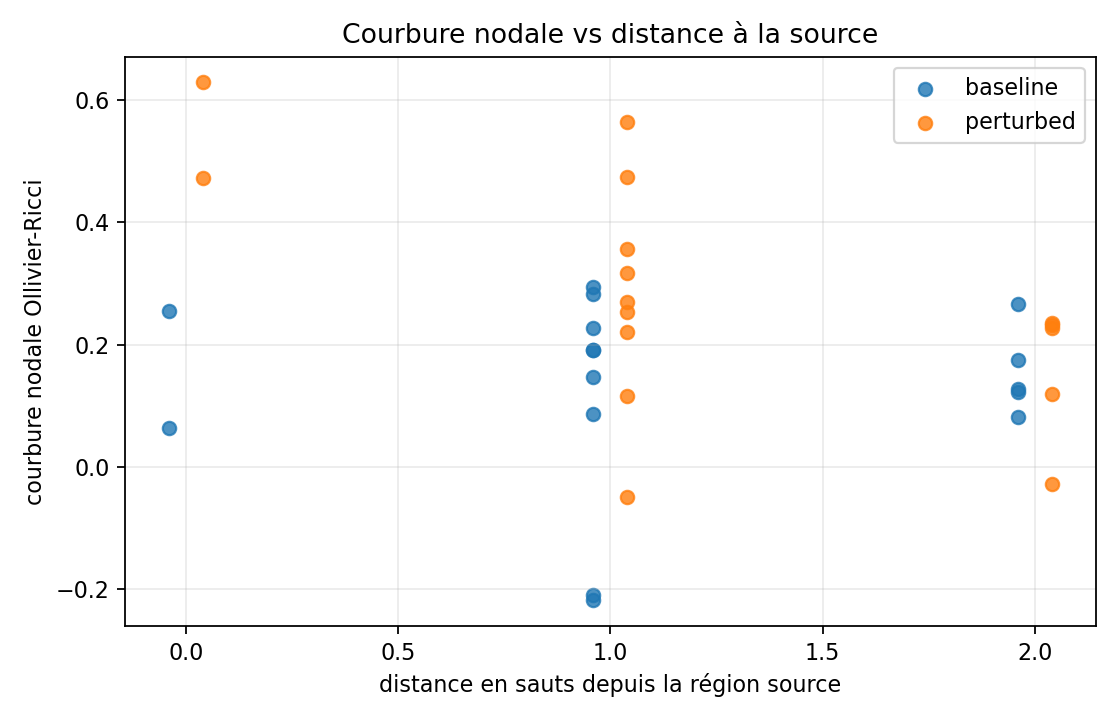
\includegraphics[width=0.72\textwidth]{../experiments/ollivier_ricci/results/v1_2_single_run/curvature_node_distance.png}
\caption{Nodal Ollivier--Ricci curvature as a function of graph distance from the source region, comparing baseline and perturbed configurations in a representative single run.}
\end{figure}

\begin{figure}[h]
\centering
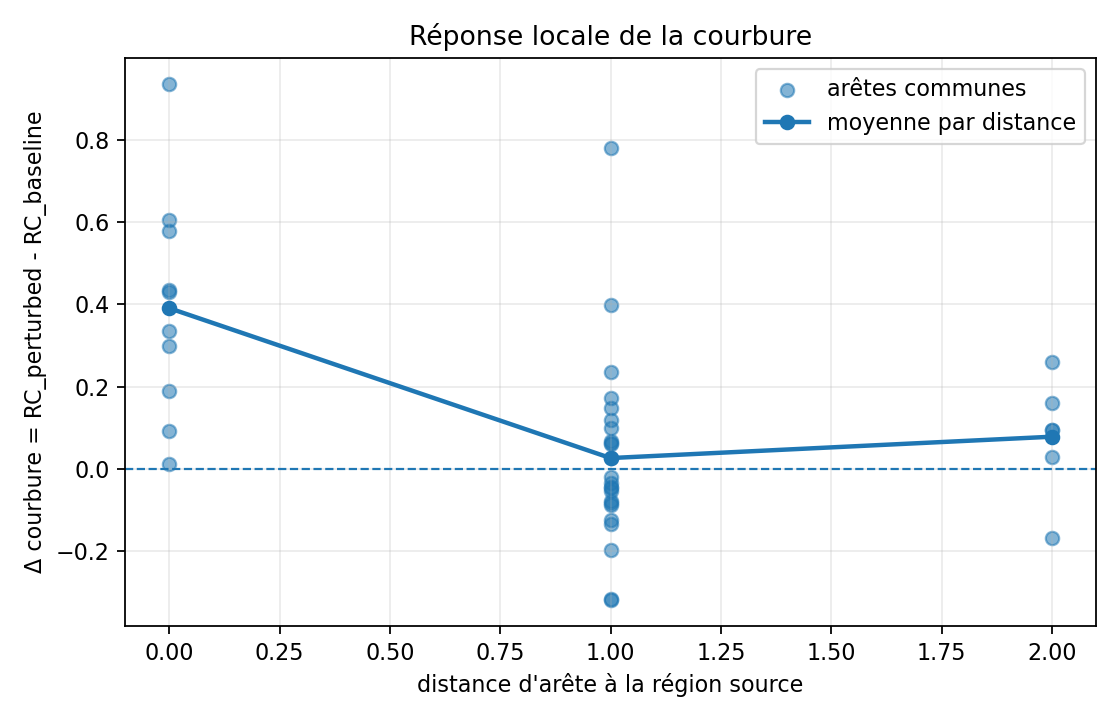
\includegraphics[width=0.72\textwidth]{../experiments/ollivier_ricci/results/v1_2_single_run/delta_edge_vs_distance.png}
\caption{Local curvature response as a function of edge distance to the source region in a representative single run. Positive values indicate an increase of curvature under the informational perturbation.}
\end{figure}

\subsection{Interpretation}

This result constitutes the clearest signal obtained so far in the project in favor of an effective coupling

\[
\text{local informational defect}
\;\Longrightarrow\;
\text{emergent geometric curvature}.
\]

This is not yet a discrete Einstein equation derived from first principles, but rather a clear numerical proof of concept showing that ``matter'' defined informationally can act as a source of curvature on the entanglement graph.

% =====================================================================
% PART VIII : SPARC PHENOMENOLOGICAL EXTENSION
% =====================================================================

\section{Phenomenological Extension: SPARC Results}

So far, the Bottom-Up program has mainly established internal signatures of emergent geometry on finite quantum systems. A decisive question is whether this effective structure can be extended to real astrophysical data.

With this in mind, we undertook a first phenomenological study on the SPARC sample of galaxy rotation curves \cite{sparc}. The aim is not yet to propose a final observational theory, but to test whether the notion of effective emergent geometry can provide a coherent descriptive framework for galactic dynamics.

\subsection{Objective}

The purpose of this analysis is to build a bridge between:

\begin{itemize}
\item emergent geometry from entanglement,
\item effective dimension,
\item large-scale gravitational response,
\item observational galaxy rotation data.
\end{itemize}

In other words, the question is whether the bottom-up program, initially formulated on finite quantum systems, can already produce a nontrivial phenomenological reading of rotation curves.

\subsection{Main result: separation into effective phases}

The most significant current result is that a strictly single-phase description does not seem optimal. The phase-diagram pipeline instead suggests the existence of distinct effective regimes.

The best fits obtained are:

\begin{center}
\begin{tabular}{ccc}
\toprule
Galactic regime & $d_{\min}$ & test $\chi^2_{\mathrm{red}}$ \\
\midrule
massive phase & $2.4871 \pm 0.0294$ & $10.9353 \pm 12.6952$ \\
dwarf phase & $2.2744 \pm 0.0341$ & $25.2842 \pm 25.8802$ \\
\bottomrule
\end{tabular}
\end{center}

These values indicate that the effective gravitational response may depend on the galactic regime, and that an emergent geometry described by a single universal dimension is not, at this stage, the most natural reading of the data.

\subsection{Provisional physical interpretation}

The current interpretation is the following:

\begin{itemize}
\item massive galaxies and dwarf galaxies may probe different effective geometric regimes;
\item emergent dimension, initially introduced as an internal observable of geometric reconstruction, acquires here a phenomenological meaning;
\item the bottom-up framework thus begins to move beyond the status of an internal model on small systems and enters an exploratory phase of confrontation with observations.
\end{itemize}

This reading remains deliberately cautious: it is a test of empirical consistency, not a definitive validation of a complete galactic model.

\subsection{Scientific status}

The SPARC part should be understood as a phenomenological proof of concept.

It does not yet constitute:

\begin{itemize}
\item a final theory of galaxy dynamics,
\item a fully constrained observational pipeline,
\item or a mature alternative to standard astrophysical fitting models.
\end{itemize}

It nevertheless represents an important step for the Bottom-Up program: emergent geometry is no longer only reconstructed internally, but is beginning to be tested against real astrophysical data.

\subsection{Scope for the Bottom-Up program}

This extension suggests that the conceptual chain

\[
\text{entanglement}
\;\Longrightarrow\;
\text{emergent geometry}
\;\Longrightarrow\;
\text{effective dimension}
\;\Longrightarrow\;
\text{gravitational response}
\]

is not only relevant at the level of finite quantum systems, but may also admit a phenomenological translation at galactic scale.

In this sense, the SPARC results constitute an important methodological advance: they open the possibility of testing bottom-up emergent geometry beyond the model's internal signatures alone.

% =====================================================================
% PART IX : SYNTHESIS AND PERSPECTIVES
% =====================================================================

\section{What the Framework Currently Establishes}

\begin{itemize}
\item geometry can emerge from finite quantum states,
\item spatial dimension depends on the entanglement structure,
\item modular dynamics is chaotic with universal RMT signatures,
\item the modular constant $C=d_A g_2^{\mathrm{plateau}}$ encodes topological information,
\item ER=EPR signatures become operationally measurable,
\item horizon-like regions emerge through informational bottlenecks,
\item a bottom-up detection algorithm identifies these regions (rank 2/55 in horizon-aware mode),
\item multipartite correlations exhibit a local triangular geometric structure,
\item triangular curvature / discrete holonomy did not provide a robust signal,
\item a local informational perturbation induces a positive Ollivier--Ricci curvature response,
\item this response grows with perturbation strength and becomes more localized for compact defects,
\item a first phenomenological extension to SPARC rotation curves suggests a description in distinct effective regimes,
\item emergent dimension, first reconstructed on finite systems, acquires a potential role as a phenomenological observable at galactic scale.
\end{itemize}

\section{Limitations}

\begin{itemize}
\item the continuum limit $N\rightarrow\infty$ is not yet established,
\item a complete relativistic dynamics is absent,
\item Einstein equations have not been derived from first principles,
\item finite system sizes limit claims of universality,
\item the modular study is limited to $|A|=8$ (other sizes remain to be explored),
\item the matter--curvature coupling is established here as a numerical proof of concept, not yet as a derived fundamental law,
\item the SPARC analysis remains exploratory and does not yet constitute a fully constrained galactic model,
\item the $\chi^2$ diagnostics indicate that further calibration and model selection work is still required.
\end{itemize}

\section{Perspectives}

Future directions include

\begin{itemize}
\item finite-size scaling toward $N>25$ (32, 36 qubits),
\item connections with SYK-type chaotic models,
\item multi-scale spectral dimension analysis,
\item random vs critical vs topological states,
\item comparison with other notions of discrete curvature,
\item derivation of an effective matter--curvature law on graphs,
\item implementations on quantum simulators,
\item experimental predictions for near-term quantum devices,
\item refinement of the galactic phase diagram on the SPARC sample,
\item testing effective laws with variable dimension according to galactic regime,
\item confrontation with other astrophysical observables: baryonic relations, lensing, mass profiles,
\item search for an effective law directly relating emergent dimension and rotation dynamics.
\end{itemize}

% =====================================================================
% CONCLUSION
% =====================================================================

\section{Conclusion}

Bottom-Up Quantum Gravity proposes that spacetime geometry can emerge from the entanglement structure of quantum states without any prior geometric background.

Even small quantum systems ($N=9,16$) display multiple coherent signatures:

\begin{itemize}
\item emergent dimension adjustable by entanglement locality, transitioning from approximately 2D for local entanglement to higher-dimensional effective geometries when nonlocal correlations dominate,
\item chaotic modular dynamics with a topology-dependent constant $C$, showing that the modular Hamiltonian spectrum retains geometric information,
\item operational ER=EPR shortcuts in which topologically distant qubits become geometrically close in the emergent metric,
\item algorithmically detectable horizon-like informational bottlenecks, with the region $\{0,2,3,5,6,10,11,15\}$ exhibiting extremely low conductance (2.7th percentile) and exceptionally high internal entanglement (98.8th percentile),
\item local geometric structure of multipartite correlations encoded by pairwise mutual informations (AUC $\approx 0.73$, $p<5\times10^{-3}$),
\item discrete triangular curvature did not yield a robust signal,
\item approximate thermodynamic gravity via a Jacobson-type entropy--energy relation,
\item local response of Ollivier--Ricci curvature to an informational perturbation, increasing with strength and more localized for compact defects,
\item a first phenomenological extension to SPARC galaxies, suggesting that distinct galactic regimes may correspond to different emergent effective dimensions.
\end{itemize}

These results suggest that spacetime may be an effective description of the informational structure of quantum states, and that several key gravitational phenomena --- including horizons and a local curvature response --- may admit a purely informational origin accessible at finite $N$. The identification of a topology-dependent modular constant $C$ provides a concrete bridge between entanglement structure and emergent geometry, while the bottom-up horizon detection algorithm offers an operational tool to identify black-hole-like regions without any prior geometric input.

The SPARC results extend this logic on the phenomenological side. Without yet constituting a complete observational theory, they suggest that an emergent geometry with variable effective dimension could provide a unifying language between bottom-up reconstruction on finite quantum systems and observed galactic dynamics. In particular, the current separation between massive and dwarf phases opens the possibility that part of the diversity of rotation curves may be interpretable in terms of distinct effective geometric regimes.

At this stage, Ollivier--Ricci curvature appears as the best discrete candidate for quantifying matter--geometry coupling in the Bottom-Up framework. It advantageously replaces the first triangular curvature diagnostics, which had not provided a sufficiently robust signal.

\begin{thebibliography}{99}

\bibitem{jacobson}
T. Jacobson,
Thermodynamics of Spacetime,
Phys. Rev. Lett. 75, 1260 (1995).

\bibitem{vanraamsdonk}
M. Van Raamsdonk,
Building up spacetime with quantum entanglement,
Gen. Relativ. Gravit. 42, 2323 (2010).

\bibitem{maldacena}
J. Maldacena, L. Susskind,
Cool horizons for entangled black holes,
Fortschritte der Physik 61, 781 (2013).

\bibitem{pagewootters}
D. Page, W. Wootters,
Evolution without evolution,
Phys. Rev. D 27, 2885 (1983).

\bibitem{ollivier}
Y. Ollivier,
Ricci curvature of Markov chains on metric spaces,
J. Funct. Anal. 256, 810--864 (2009).

\bibitem{sparc}
F. Lelli, S. S. McGaugh, J. M. Schombert,
SPARC: Mass Models for 175 Disk Galaxies with Spitzer Photometry and Accurate Rotation Curves,
Astron. J. 152, 157 (2016).

\end{thebibliography}

\end{document}
